\documentclass[xcolor={dvipsnames},aspectratio=169,10pt]{beamer}

% utility packages
\usepackage{etoolbox}
\usepackage{multicol}
\usepackage{relsize}
\usepackage{fontawesome}

% better text justifying
\usepackage{microtype}
% justify text inside list environment
% Ref: http://liam0205.me/2017/04/11/justifying-in-beamer-s-lists/
\usepackage{ragged2e}
\makeatletter
\patchcmd{\itemize}{\raggedright}{\justifying}{}{}
\patchcmd{\beamer@enum@}{\raggedright}{\justifying}{}{}
\patchcmd{\@@description}{\raggedright}{\justifying}{}{}
\makeatother

% math related packages
\usepackage{amsmath}
\usepackage[ruled,vlined]{algorithm2e}
\SetAlCapNameFnt{\scriptsize}
\SetAlCapFnt{\scriptsize}
\SetAlFnt{\scriptsize}

% figure related packages
\usepackage{graphicx}
\usepackage[scale=2]{ccicons}
\usepackage{qrcode}
\usepackage{tikz}
\usepackage{tikzpagenodes}
\usetikzlibrary{positioning}

% table related packages
\usepackage{array}
\usepackage{booktabs}
\usepackage{multirow}
\usepackage{colortbl}
\newcommand{\tabincell}[2]{\begin{tabular}{@{}#1@{}}#2\end{tabular}}

% code highlight
\usepackage{listings}
\usepackage{minted}
\definecolor{mintedbg}{HTML}{E5E9F0}
\setminted{autogobble,bgcolor=mintedbg,fontsize=\small}
\setmintedinline{bgcolor=mintedbg,fontsize=\smaller}
\newminted{bash}{}
\newminted{latex}{}
\newmintinline{bash}{}
\newmintinline{latex}{}
\newcommand{\texdoc}[2]{\href{#2}{\bashinline|texdoc #1|}}

% hyperref setting
\hypersetup{
  unicode,
  psdextra,
  bookmarksnumbered=true,
  bookmarksopen=true,
  bookmarksopenlevel=3,
  bookmarksdepth=4,
  pdfcenterwindow=true,
  pdfstartview={Fit},
  pdfpagemode={FullScreen},
  pdfpagelayout={SinglePage},
}
\usepackage{bookmark}

% beamer theme
\usetheme{metropolis}
\metroset{block=fill,numbering=fraction}

% caption style
\usepackage{subcaption}
\setlength\abovecaptionskip{3pt}
\setbeamerfont{caption}{size=\scriptsize}
\renewcommand{\figurename}{Fig.}
\captionsetup{labelformat=empty,labelsep=none,textfont={bf,it}}

% Ref: https://github.com/gpoore/minted/blob/master/source/minted.dtx
\newenvironment{latexexample}
{\VerbatimEnvironment\begin{VerbatimOut}[gobble=3]{example.out}}{\end{VerbatimOut}%
  \begin{center}
    \begin{minipage}{0.47\linewidth}%
      \inputminted[resetmargins,fontsize=\scriptsize]{latex}{example.out}%
    \end{minipage}%
    \hspace{0.05\linewidth}%
    \begin{minipage}{0.47\linewidth}%
      \begin{framed}
        \setlength{\parindent}{2em}%
        \input{example.out}%
      \end{framed}
    \end{minipage}%
  \end{center}
}

\newenvironment{mathexample}
{\VerbatimEnvironment\begin{VerbatimOut}[gobble=3]{example.out}}{\end{VerbatimOut}%
  \begin{center}
    \begin{minipage}{0.47\linewidth}%
      \inputminted[resetmargins,fontsize=\scriptsize]{latex}{example.out}%
    \end{minipage}%
    \hspace{0.05\linewidth}%
    \begin{minipage}{0.47\linewidth}%
      \begin{framed}
        \[ \input{example.out} \]
      \end{framed}
    \end{minipage}%
  \end{center}
}

\newenvironment{mathexamples}
{\VerbatimEnvironment\begin{VerbatimOut}[gobble=3]{example.out}}{\end{VerbatimOut}%
  \begin{center}
    \begin{minipage}{0.47\linewidth}%
      \inputminted[resetmargins,fontsize=\scriptsize]{latex}{example.out}%
    \end{minipage}%
    \hspace{0.05\linewidth}%
    \begin{minipage}{0.47\linewidth}%
      \begin{framed}
        \directlua{
          local first = true
          for line in io.lines('example.out') do
          if first then
          first = false
          else
          tex.print('\\newline ')
          end
          tex.print('$' .. line .. '$')
          end
        }
      \end{framed}
    \end{minipage}%
  \end{center}
}


\title{The Future of Engineering}
\subtitle{Challenges and opportunities }
\author{Miguel Xochicale  (\faGithub @mxochicale  \faTwitter @\_mxochicale) 
}
\date{October 21, 2020}
\titlegraphic{
  \begin{tikzpicture}[overlay, remember picture]
    \node[%
      above right=0.35cm and -0.2cm of current page footer area.south west,
      anchor=south west,
      inner sep=0pt] {%
      \usebeamerfont{footline}
      \begin{tabular}{lm{.8\textwidth}}
        \href{http://creativecommons.org/licenses/by/4.0/}{\ccby} &
        This work is licensed under a 
	\href{http://creativecommons.org/licenses/by/4.0/}
		{Creative Commons ``Attribution 4.0 International''} license. 
	\par Get source of this slides and see further references from \url{https://github.com/mxochicale/itds2020}.
      \end{tabular}
    };
    \node[%
      above left=0.35cm and 0cm of current page footer area.south east,
      anchor=south east,
      inner sep=0pt]{\qrcode[height=1.5cm]{https://github.com/mxochicale/}};
  \end{tikzpicture}
}

\begin{document}

\maketitle%

\begin{frame}{Contents}
  \setbeamertemplate{section in toc}[sections numbered]
  \tableofcontents[hideallsubsections]
\end{frame}


%%%%%%%%%%%%%%%%%%%%%%%%%%%%%%%%%%%%%%%%%%%%
\section{Short-bio}

\begin{frame}{My journey in Engineering and Science}

\begin{itemize}	
	\item \textbf{(1996-1999)} Hight School in Electronics
	\item \textbf{(1999-2004)} BSc in Electronics  
	\item \textbf{(2004-2006)} MSc in Signal Processing 
	\item \textbf{(2006-2012)} Teaching Associate in Mechatronics 
	\item \textbf{(2013-2014)} Research Assistant in Robotics at INAOE  
	\item \textbf{(2014-2019)} PhD student in Human-Robot Interaction at Uni of Bham \\
	\item \textbf{(2019-present)} Research Associate in Ultrasound-Guidance 
	Intervention at KCL 
\end{itemize}

	\vspace{4mm}
        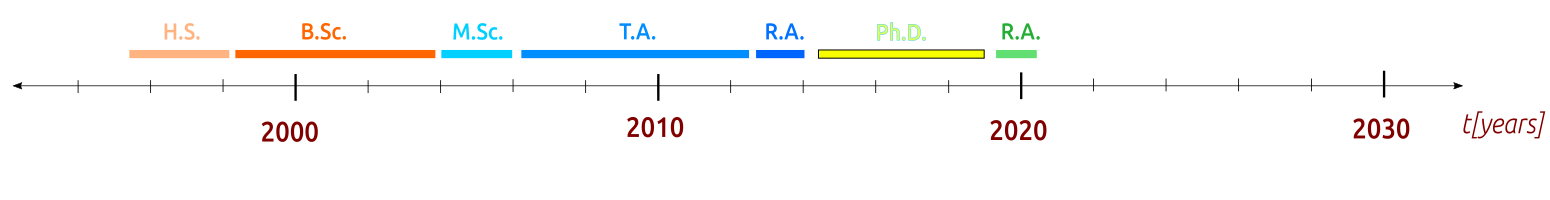
\includegraphics[width=\linewidth]{./figs/myjourney/versions/drawing.png}

\end{frame}

\begin{frame}[fragile]{Installation}
  \begin{itemize}
    \item \textbf{Windows/Linux}
          \begin{itemize}
            \item TeXLive \url{https://www.tug.org/texlive/}
            \item Online installer:
                  \begin{itemize}
                    \item Windows \\ \url{http://mirror.ctan.org/systems/texlive/tlnet/install-tl-windows.exe}
                    \item Linux \\ \url{http://mirror.ctan.org/systems/texlive/tlnet/install-tl-unx.tar.gz}
                  \end{itemize}
            \item Offline ISO file:
                  \footnotesize
                  \url{http://mirror.ctan.org/systems/texlive/Images/}
          \end{itemize}
    \item \textbf{Mac}
          \begin{itemize}
            \item MacTeX \url{http://www.tug.org/mactex/}
            \item Or install through Homebrew (\url{https://brew.sh}) \\
                  \begin{minipage}{\linewidth+2.1em}
                    \inputminted[fontsize=\scriptsize]{bash}{./minted/install_mactex.sh}
                    \vspace{-2ex}
                  \end{minipage}
          \end{itemize}
    \item TeXLive/MacTeX release major updates around May each year. \\
          It is recommended to uninstall the old version and install the new version annually.
  \end{itemize}
\end{frame}

\begin{frame}{\LaTeX~editor}
  \begin{itemize}
    \item \LaTeX~source codes are plaintext. So you can use any editor you like.
    \item \textbf{Visual Studio Code \alert{[Recommend]}}
          \begin{itemize}
            \item \footnotesize \url{https://code.visualstudio.com}
            \item LaTeX Workshop \footnotesize \url{https://github.com/James-Yu/LaTeX-Workshop}
            \item Code Spell Checker \footnotesize \url{https://github.com/streetsidesoftware/vscode-spell-checker}
          \end{itemize}
    \item \textbf{Vim/Neovim}
          \begin{itemize}
            \item \footnotesize \url{https://www.vim.org} | \url{https://neovim.io}
            \item Vimtex \footnotesize \url{https://github.com/lervag/vimtex}
          \end{itemize}
    \item \textbf{Emacs}
          \begin{itemize}
            \item \footnotesize \url{https://www.gnu.org/s/emacs}
            \item AUCTeX \footnotesize \url{https://www.gnu.org/software/auctex}
          \end{itemize}
    \item \textbf{TeXstudio}
          \begin{itemize}
            \item \footnotesize \url{https://www.texstudio.org}
          \end{itemize}
  \end{itemize}
\end{frame}


%%%%%%%%%%%%%%%%%%%%%%%%%%%%%%%%%%%%%%%%%%%%
\section{Challenges and Opportunities in Engineering}
\begin{frame}[fragile]{Hello, \LaTeX!}
  \begin{columns}
    \begin{column}{.7\linewidth}
      \begin{itemize}
        \item Create \mintinline{text}|hello.tex| file with following content.
              \inputminted{latex}{./minted/hello.tex}
        \item Compile it
              \begin{itemize}
                \item Click the build button in your \LaTeX~editor/IDE
                \item OR using command line: \bashinline|latexmk -pdf hello|
              \end{itemize}
        \item Open \mintinline{text}|hello.pdf| to preview the result
      \end{itemize}
    \end{column}
    \begin{column}{.3\linewidth}
      \begin{figure}
        \centering
        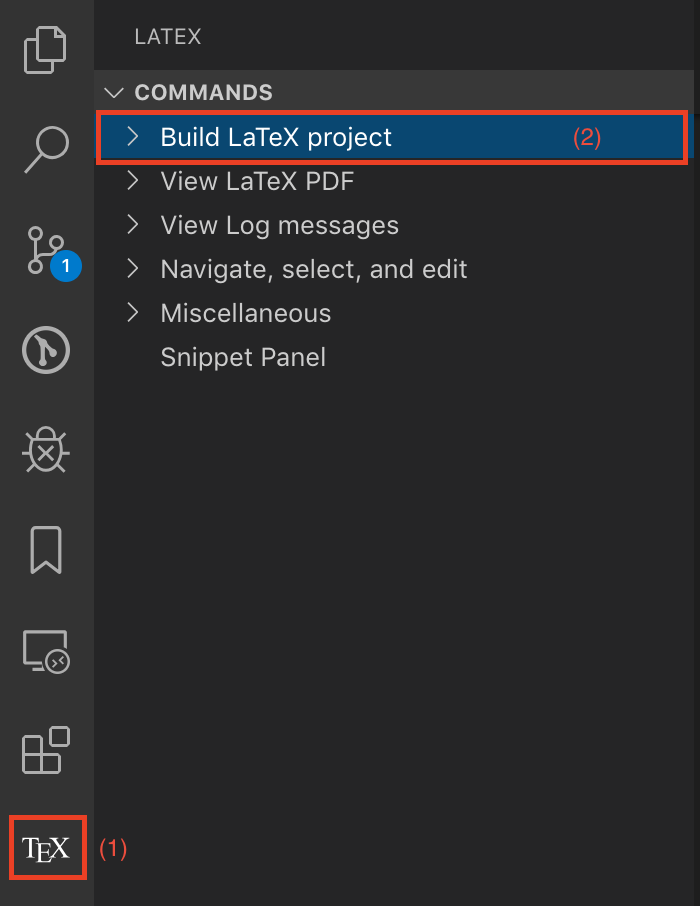
\includegraphics[width=\linewidth]{./figs/vscode-compile-project.png}
        \caption{Compile \LaTeX~Project in VSCode}
      \end{figure}
    \end{column}
  \end{columns}
\end{frame}

\begin{frame}[fragile]{Example of A Complex Document}
  \begin{itemize}
    \item Download the source code from \url{https://github.com/xu-cheng/latex-tutorial/archive/master.zip}
    \item The example document is located in the \mintinline{text}|example| folder. It contains:
          \begin{itemize}
            \item \mintinline{text}|main.tex| The main tex source
            \item \mintinline{text}|preamble.tex| A subfile to store format definitions
            \item \mintinline{text}|tikz-example.tex| A figure drawn using tikz
            \item \mintinline{text}|ref.bib| A database of references
          \end{itemize}
    \item Use \bashinline|latexmk -pdf main| to compile the document
    \item Access the same example in Overleaf: \url{https://www.overleaf.com/read/qsthqbjphhrz}
  \end{itemize}
\end{frame}

% \begin{noindent}
\begin{frame}[fragile]{Comment, Command and Environment}
  \begin{itemize}
    \item \latexinline|%| starts a comment. e.g.~\latexinline|% this is hello.tex|
    \item \latexinline|\| starts a command.
          \begin{latexcode}
            \command % a command
            \command{} % also a command
            \command{arg} % a command with an argument
            \command{arg1}{arg2} % a command with multiple arguments
            \command[opt arg]{arg} % [] is for optional argument
          \end{latexcode}
    \item \latexinline|\begin{} ... \end{}| denotes an environment
          \begin{latexcode}
            \begin{envname}
              inside the environment
            \end{envname}
            % LaTeX environment can take arguments
            \begin{envname}{arg} \end{envname}
            \begin{envname}[opt arg]{arg} \end{envname}
          \end{latexcode}
  \end{itemize}
\end{frame}
% \end{noindent}

\begin{frame}[fragile]{Source File Structure}
  \begin{itemize}
    \item A document starts with \latexinline|\documentclass{...}| command to specify the template
    \item Common templates include:
          \setlength{\multicolsep}{0pt}
          \setlength{\columnsep}{0pt}
          \begin{multicols}{3}
            \begin{itemize}
              \item \texttt{article}
              \item \texttt{book}
              \item \texttt{report}
              \item \texttt{letter}
              \item \texttt{beamer} \textsmaller{(slides)}
              \item \texttt{standalone} \textsmaller{(graphics)}
              \item \texttt{acmart} \textsmaller{(ACM~template)}
              \item \texttt{IEEEtrans} \textsmaller{(IEEE~template)}
              \item[]
            \end{itemize}
          \end{multicols}
    \item Template class can accept options, e.g.~\latexinline|\documentclass[a4paper,10pt]{article}|
  \end{itemize}

  \begin{block}{Class Options for \texttt{article}, \texttt{report}, \texttt{book}, \texttt{letter}}
    \begin{description}[\scriptsize\texttt{titlepage}, \texttt{notitlepage}]
      \scriptsize
      \item[\normalfont\texttt{10pt}, \texttt{11pt}, \texttt{12pt}] \quad Set font size.
      \item[\normalfont\texttt{a4paper}, \texttt{letterpaper}, \ldots] \quad Defines
            the paper size.
      \item[\normalfont\texttt{fleqn}] \quad Typesets displayed formulae left-aligned
            instead of centred.
      \item[\normalfont\texttt{leqno}] \quad Places the numbering of formulae on the
            left hand side instead of the right.
      \item[\normalfont\texttt{titlepage}, \texttt{notitlepage}] \quad Specifies whether a new page should be started after the document title or not.
      \item[\normalfont\texttt{onecolumn}, \texttt{twocolumn}] \quad Typeset the document in one column or two columns.
      \item[\normalfont\texttt{twoside, oneside}] \quad Specifies whether double or single sided output should be generated.
      \item[\normalfont\texttt{landscape}] \quad Changes the layout of the document to print in landscape mode.
      \item[\normalfont\texttt{openright, openany}] \quad Makes chapters begin either only on right hand pages or on the next page available.
    \end{description}
  \end{block}
\end{frame}


%%%%%%%%%%%%%%%%%%%%%%%%%%%%%%%%%%%%%%%%%%%%
\section{Engineering as Multidisciplinary Field}

\begin{frame}{Introduction}
  \begin{itemize}
    \item \alert{\LaTeX{}} is a document preparation system and document markup language.
    \item It can be used to typeset articles, books, slides, posters, even graphics.
    \item \textbf{\textcolor{Green}{Pros}:}
          \begin{itemize}
            \item It separates presentation/format from contents.
            \item Since the source codes are plaintext, it works well with version control system such as git.
            \item Highly customizable through various of packages.
          \end{itemize}
    \item \textbf{\textcolor{Red}{Cons}:}
          \begin{itemize}
            \item There is no graphic interface to support WYSIWYG style editing.
            \item Not suitable to produce unstructured documents.
          \end{itemize}
  \end{itemize}
\end{frame}


%%%%%%%%%%%%%%%%%%%%%%%%%%%%%%%%%%%%%%%%%%%%
\section{Robotics Engineering and open-source projects}

\begin{frame}{Introduction}
  \begin{itemize}
    \item \alert{\LaTeX{}} is a document preparation system and document markup language.
    \item It can be used to typeset articles, books, slides, posters, even graphics.
    \item \textbf{\textcolor{Green}{Pros}:}
          \begin{itemize}
            \item It separates presentation/format from contents.
            \item Since the source codes are plaintext, it works well with version control system such as git.
            \item Highly customizable through various of packages.
          \end{itemize}
    \item \textbf{\textcolor{Red}{Cons}:}
          \begin{itemize}
            \item There is no graphic interface to support WYSIWYG style editing.
            \item Not suitable to produce unstructured documents.
          \end{itemize}
  \end{itemize}
\end{frame}




%%%%%%%%%%%%%%%%%%%%%%%%%%%%%%%%%%%%%%%%%%%%
\section{The Future Engineering }

\begin{frame}{Introduction}
  \begin{itemize}
    \item \alert{\LaTeX{}} is a document preparation system and document markup language.
    \item It can be used to typeset articles, books, slides, posters, even graphics.
    \item \textbf{\textcolor{Green}{Pros}:}
          \begin{itemize}
            \item It separates presentation/format from contents.
            \item Since the source codes are plaintext, it works well with version control system such as git.
            \item Highly customizable through various of packages.
          \end{itemize}
    \item \textbf{\textcolor{Red}{Cons}:}
          \begin{itemize}
            \item There is no graphic interface to support WYSIWYG style editing.
            \item Not suitable to produce unstructured documents.
          \end{itemize}
  \end{itemize}
\end{frame}




\begin{frame}[standout]
  Thanks \\
  Questions?
\end{frame}

\end{document}
